\documentclass[12pt]{article}
\usepackage{amsmath}
\usepackage{hyperref}
\usepackage{graphicx}

\title{Non-Perturbative QFT Problem Sheet - Question 4}
\author{Matthew Hawes}
\date{\today}


\begin{document}
\maketitle

\begin{abstract}
This question is in two sections, firstly a description of the algorithm used followed by the results of the simulations. Full code is available at \url{www.github.com\\mghawes}.
\end{abstract}

\section{Algorithm}
The algorithm, implemented in C++, relies heavily on the concept of Object-Oriented programing to improve readability as well as speed. The general principal in this case being to create objects with methods and attributes that can be initialized once and then iterated on very efficiently. The key point being that we do as much setup as possible \emph{before} beginning to perform the metropolis updates. The simplest example of this is the abstraction of the lattice, which will now describe as a primer.

\subsection{Lattice}
The most efficient way to store a $U(1)$ lattice is to store the phases $\theta_l$ of the group elements $U_l = \mathrm{e}^{i\theta_l}$ that live on the links $l$. In memory these links will exist as just a contiguous block,or array, of \texttt{double} values. Thus, we have to prescribe some mapping from the $2+1\mathrm{D}$ lattice to the elements of the $1\mathrm{D}$ array. The mapping chosen is to split the array into three blocks with the first third containing only $x$ directed links and the 2nd and 3rd containing $y$ and $t$ links. Within each of these blocks we `unravel' the lattice into a $1\mathrm{D}$ array by moving first along the $x$ direction, then moving along $y$ and finally along $z$. This is depicted in Fig~\ref{fig:latticeunpack}


\begin{figure}
\centering
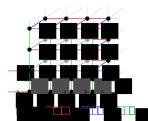
\includegraphics[width=0.6\linewidth]{latticeunpack.png}
\caption{'Unraveling' the links of the lattice into a $1\mathrm{D}$ array depicted beneath the lattice. Rights belong to the author.}
\label{fig:latticeunpack}
\end{figure}


\section{Results}
In this section we describe the results.


\end{document}